\begin{frame}{Environment (Parallel-Split Shadow Maps)}
%
\begin{itemize}
	\item Crucial para obtener sombras de calidad.
	\item Crítico en función de la distancia mínima de corte:
	\[
	\left( \begin{matrix} x_v \\ y_v \\ z_v \\ w_v \end{matrix} \right)	
	=
	\left( \begin{matrix} 
		\frac{n}{r} & 0           & 0                & 0                  \\
		0           & \frac{n}{h} & 0                & 0                  \\
		0           & 0           & -\frac{f+n}{f-n} & -\frac{2 f n}{f-n} \\
		0           & 0           & -1               & 0                  \\
	\end{matrix} \right)	
	\left( \begin{matrix} x \\ y \\ z \\ w \end{matrix} \right)	
	,
	\]
	Resultando la profundidad del punto en pantalla como:
	\[ z_s = \frac{z_v}{w_v} = 2 \frac{f n}{f - n} \frac{w}{z} + \frac{f + n}{f - n}
	= \mathcal{O}\left( \frac{1}{z} \right) \]
\end{itemize}
\pause
\hrule
\vspace{0.2cm}
%
\begin{columns}
  \begin{column}{0.5\textwidth}
    \textbf{\underline{Blender}} (\textcolor{red}{-98} líneas)
    
    \vspace{1.2cm}
    Implementado internamente en el motor de Blender.
  \end{column}

  \begin{column}{0.5\textwidth}
    \textbf{\underline{OGRE}} (\textcolor{red}{-1054-379-159} líneas)
        
    \vspace{0.5cm}
    \begin{tikzpicture}[scale=0.8]
    	\node [whitebox] (Header file) at ($(-5,\vertspacing*1)$) {
    		\nodelabel{Header file}{\textit{40 líneas}}
    	};
    	\node [whitebox] (Source file) at ($(-5,\vertspacing*2)$) {
    		\nodelabel{Source file}{\textit{119 líneas}}
    	};
    \end{tikzpicture}    
  \end{column}
\end{columns}
\end{frame}

\begin{frame}{Environment (Atmósfera)}
\begin{columns}
  \begin{column}{0.5\textwidth}
    \textbf{\underline{Blender}} (\textcolor{red}{-98} líneas)
    
    \vspace{0.4cm}
    La cámara no permite apreciar la atmósfera, y por tanto no ha sido implementada.
  \end{column}

  \begin{column}{0.5\textwidth}
    \textbf{\underline{OGRE}} (\textcolor{red}{-1054-379-159-11877} líneas)
    
    \vspace{0.4cm}
    \begin{tikzpicture}[scale=0.8]
    	\node [whitebox] (SkyX) at ($(-5,\vertspacing*1)$) {
    		\nodelabel{SkyX}{\textit{11877 líneas}}
    	};
    \end{tikzpicture}    
  \end{column}
\end{columns}
\begin{figure}
	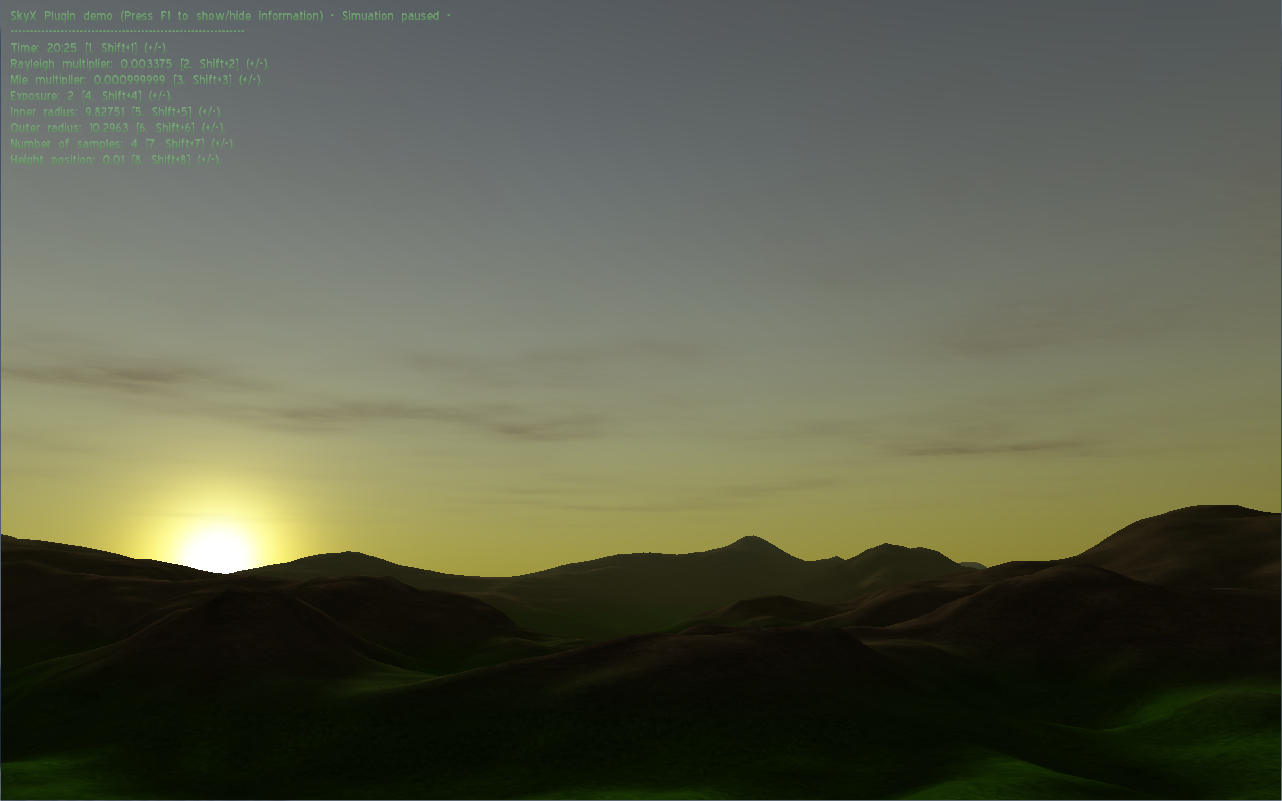
\includegraphics[scale=0.1]{skyx_sky} 
	
\includegraphics[scale=0.2095]{skyx_clouds} 
\end{figure}
\end{frame}

\begin{frame}{Environment (Océano)}
\begin{columns}
  \begin{column}{0.5\textwidth}
    \textbf{\underline{Blender}} (\textcolor{red}{-98-38} líneas)
    
    \vspace{0.4cm}
    \begin{tikzpicture}[scale=0.8]
    	\node [whitebox] (Plano) at ($(-5,\vertspacing*1)$) {
    		\nodelabel{Plano que sigue a la cámara}{\textit{38 líneas}}
    	};
    	\node [whitebox] (Olas) at ($(-5,\vertspacing*2)$) {
    		\nodelabel{Olas creadas internamente en el shader}{\textit{0 líneas}}
    	};
    	\node [whitebox] (Submarino) at ($(-5,\vertspacing*3)$) {
    		\nodelabel{Sin entorno submarino}{\textit{0 líneas}}
    	};
    \end{tikzpicture}
  \end{column}

  \begin{column}{0.5\textwidth}
    \textbf{\underline{OGRE}} (\textcolor{red}{-1054-379-159-11877-8220} líneas)
    
    \vspace{0.4cm}
    \begin{tikzpicture}[scale=0.8]
    	\node [whitebox] (Geometría compleja) at ($(-5,\vertspacing*1)$) {
    		\nodelabel{Geometría compleja}{\textit{121+159+193+229+277+452+667+842 líneas}}
    	};
    	\node [whitebox] (Olas) at ($(-5,\vertspacing*2)$) {
    		\nodelabel{Olas generadas sobre la geometría}{\textit{65+97+112+133+135+152+186+194+272+282+589+800 líneas}}
    	};
    	\node [whitebox] (Submarino) at ($(-5,\vertspacing*3)$) {
    		\nodelabel{Entorno submarino}{\textit{$\sim$43+$\sim$75+335+$\sim$190+$\sim$255+915+$\sim$450 líneas}}
    	};
    \end{tikzpicture}
  \end{column}
\end{columns}
\begin{figure}
	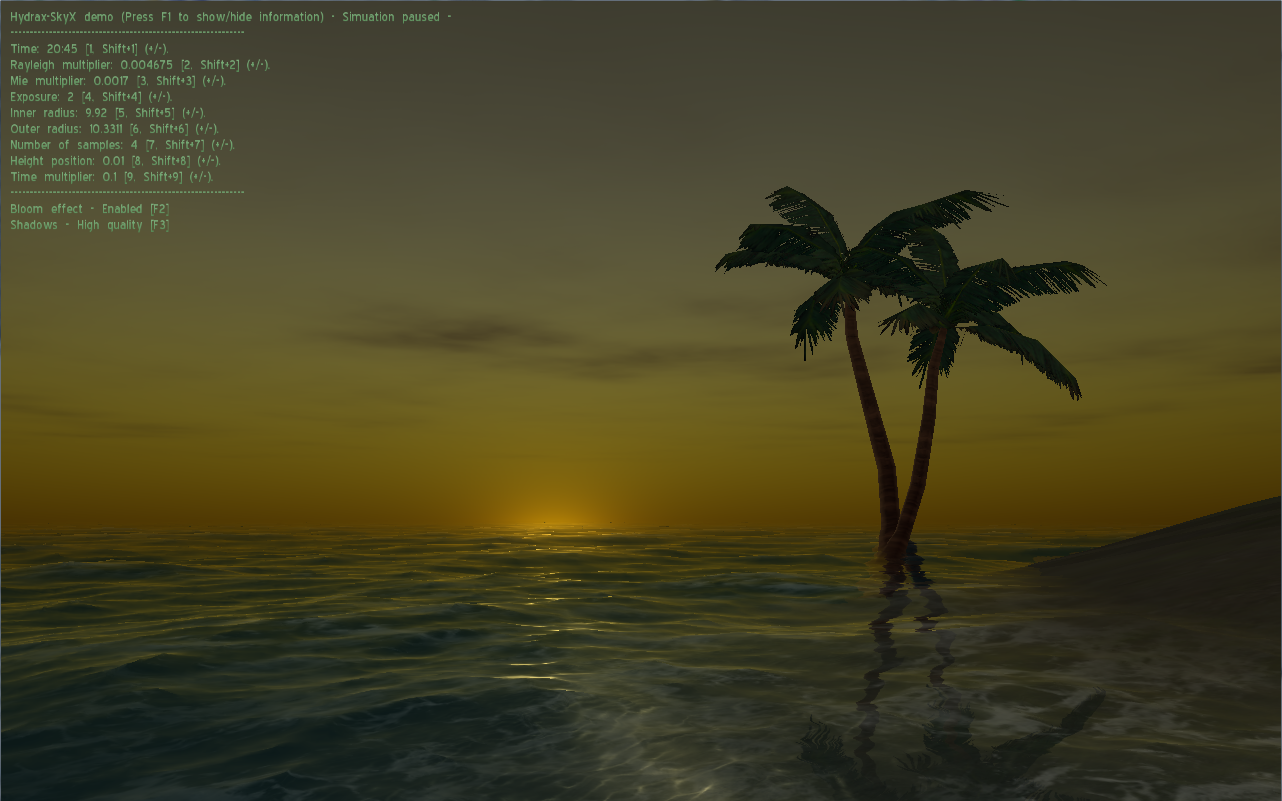
\includegraphics[scale=0.15]{hydrax} 
\end{figure}
\end{frame}
